% ===================================================================
%  Αρχείο: 15617_tikz.tex (Fragment)
%  Αυτόματη μετατροπή μέσω doc2latex.py & TikZ conversion
% ===================================================================

ΘΕΜΑ 2

Δίνεται η συνάρτηση $f(x) = \ln\frac{1}{|x|}$ , $x\mathbb{\in R - \{}0\}$ .

\begin{alist}
\item Να αποδείξετε ότι $f(x) = - \ln|x|$, για κάθε $x\mathbb{\in R - \{}0\}$ .

\monades{10}

\item i) Στο παρακάτω σχήμα δίνεται η γραφική παράσταση της συνάρτησης $h(x) = \ln|x|,$ $x\mathbb{\in R - \{}0\}$.

\begin{center}
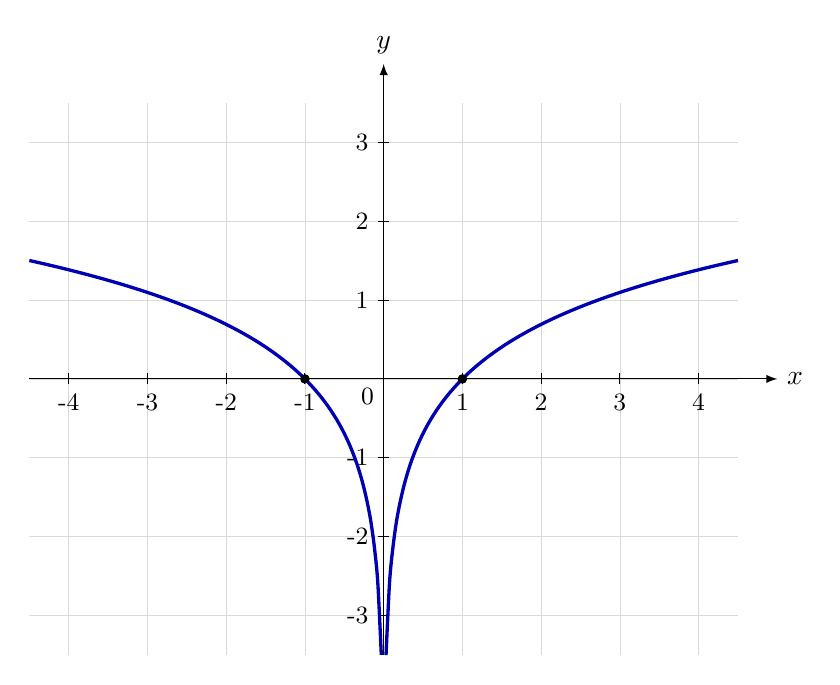
\begin{tikzpicture}[scale=1, >=latex]
    \draw[very thin, color=gray!30] (-4.5,-3.5) grid (4.5,3.5);
    \draw[->] (-4.5,0) -- (5,0) node[right] {$x$};
    \draw[->] (0,-3.5) -- (0,4) node[above] {$y$};
    
    \foreach \x in {-4,-3,-2,-1,1,2,3,4}
        \draw (\x,2pt) -- (\x,-2pt) node[below, font=\small] {\x};
    \foreach \y in {-3,-2,-1,1,2,3}
        \draw (2pt,\y) -- (-2pt,\y) node[left, font=\small] {\y};
    \node[below left, font=\small] at (0,0) {$0$};
    
    % h(x) = ln|x|
    \draw[very thick, color=blue!70!black, samples=100, smooth, domain=0.03:4.5] plot (\x, {ln(\x)});
    \draw[very thick, color=blue!70!black, samples=100, smooth, domain=-4.5:-0.03] plot (\x, {ln(-\x)});
    
    % Roots
    \filldraw (1,0) circle (1.5pt);
    \filldraw (-1,0) circle (1.5pt);
\end{tikzpicture}
\end{center}

Να σχεδιάσετε τη γραφική παράσταση της συνάρτησης $f.$

\monades{7}

ii) Να αποδείξετε ότι οι γραφικές παραστάσεις των $f$ και $g(x) = \ln x,x > 0$ έχουν μοναδικό κοινό σημείο για $x = 1.$

\monades{8}
\end{alist}
